% Preamble
\documentclass[xcolor=dvipsnames]{beamer}
\usetheme{madrid}

% Packages
\usepackage[english,ngerman]{babel}
\usepackage[utf8]{inputenc}
\usepackage{amsmath}
\usepackage{graphicx}
\usepackage{ifthen} % Boolean variables
\usepackage{subfigure} % Horizontal pictures

\definecolor{hBlue}{RGB}{55,118,165}
\usecolortheme[named=hBlue]{structure}

% Distiction between work and stream presentation
\newboolean{work}
\setboolean{work}{true}

\ifthenelse{\boolean{work}}{
    \titlegraphic{
\includegraphics[width=4cm]{../images/logo.png}}
}{}
\title{Gesundheit \& Ernährung}
\subtitle{Mayr-Medizin}
\ifthenelse{\boolean{work}}{
    \author{Adrian Helberg}
}{
    \author{Bl1nzlar, twitch.tv/bl1nzlar}
}
\date{11.08.2021}


% Document
\begin{document}

    \maketitle

    \frame{\frametitle{Agenda}\tableofcontents}

    \section{Theorie}
    {
    \setbeamercolor{normal text}{fg=hBlue}\usebeamercolor*{normal text}
    \begin{frame}
        \begin{center}
            \Huge Theorie
        \end{center}
    \end{frame}
    }

    \subsection{Profil}
    \begin{frame}[allowframebreaks]
        \frametitle{Profil}

        \begin{block}{Franz Xaver Mayr}
            \begin{itemize}
                \setlength\itemsep{1em}
                \item 1875–1965
                \item Kurarzt in der Steiermark, in Karlsberg und Wien
                \item \textit{"`Die meisten gesundheitlichen Störungen hängen mit dem Darm zusammen"'}
                \item Therapie \textit{Milch-Semmel-Kur}
                \item Die Art der Ernährung ist mindestens so wichtig wie das Nahrungsmittel selbst
            \end{itemize}
        \end{block}

        \famebreak

        \begin{block}{Internationalen Gesellschaft der Mayr-Ärzte}
            \begin{itemize}
                \setlength\itemsep{1em}
                \item Sitz im Geburtshaus von Dr. F.X. Mayr in Gröbming, Österreich
                \item Diagnose- und Therapieverfahren zur Behandlung chronischer Erkrankungen und zur Gesundheitsvorsorge
                \item Ausbildung und Zertifizierung von Ärzten zu diplomierten Mayr-Ärzten
            \end{itemize}
        \end{block}
    \end{frame}

    \subsection{Der Gesundheitsbegriff}
    \begin{frame}[allowframebreaks]
        \frametitle{Der Gesundheitsbegriff nach F.X.Mayr}

        \begin{block}{Optimale Gesundheit}
            \begin{itemize}
                \setlength\itemsep{1em}
                \item "`Moderne Medizin"' orientiert sich an Normwerten einer subjektiv beschwerdefreien Durschnittsbevölkerung
                \item \textit{"`Wer will schon ein Durchschnittsgebiss haben?"'}
                \item Optimale Gesundheit sollte ein Zustand sein, der sich nicht weiter verbessern lässt
                \item Ganzheitliche Betrachtung des Menschen (keine Trennung von Knochen-, Muskelsystem, etc.)
            \end{itemize}
        \end{block}

        \framebreak

        \begin{block}{Kennzeichen des/der optimal-gesunden \ldots}
            \begin{itemize}
                \setlength\itemsep{1em}
                \item Abdomens (Bauch)
                \item Körperhaltung
                \item Körpersäfte
                \item Haut
            \end{itemize}
        \end{block}

        \begin{block}{Gesundheitszustände}
            \begin{itemize}
                \item Optimal
                \item Suboptimal
                \item Durchschnittlich
                \item Noch nicht krank
                \item Krank
            \end{itemize}
        \end{block}
    \end{frame}

    \subsection{Mayr-Medizin}
    \begin{frame}[allowframebreaks]
        \frametitle{Mayr-Medizin}

        \begin{block}{Was ist "`Mayr-Medizin"'}
            \begin{itemize}
                \setlength\itemsep{1em}
                \item Ganzheitliche Methode zur Verbesserung der Gesundheit
                \item Verbesserung aller Organfunktionen und der Lebensqualität
                \item Ärztliche Diagnostik und Therapie (ca. 3 Wochen) durch
                \begin{itemize}
                    \item Schonung
                    \item Säuberung
                    \item Schulung
                    \item Substitution (Moderne Mayr-Medizin)
                \end{itemize}
                \item Alle Säulen der Therapie werden gleichzeitig und individuell angewendet
            \end{itemize}
        \end{block}

        \begin{block}{Motivation - Fehler der "`Ernährungs-Pipeline"'}
            \begin{itemize}
                \setlength\itemsep{1em}
                \item \textbf{Zu schnell}: Keine Vorverdauung, zu wenig Spülspeichel
                \item \textbf{Zu viel}: Überlastung mit Energie, Nährstoffresorption findet im ersten Drittel des Darms statt, zu viel Nahrung darüber hinaus
                \item \textbf{Zu oft}: Keine Grob- und Feinsäuberung (ab 4-6h Essenspause) des Darms mehr möglich, Überbelastung der Bauchspeicheldrüse
                \item \textbf{Zu spät}: Keine vollständige Verdauung möglich, da Tageszeitenabhängig
                \item \textbf{Zu schwer}: Keine vollständige Resorption möglich (Konstitutionsabhängigkeit, Vitalitätszustand)
            \end{itemize}
        \end{block}

        \begin{block}{Diagnostik}
            \begin{itemize}
                \setlength\itemsep{1em}
                \item \textbf{Körperhaltung}
                \item \textbf{Bauchformen}
                \item \textbf{Schmerzempfindlichkeit} der Bauchdecke
                \item \textbf{Körpermaße} von Brustkorb, Bauch, Hals, etc.
                \item \textbf{Beschaffenheit} von Haut, Haaren, etc.
            \end{itemize}
        \end{block}
    \end{frame}

    \subsection{Intestinale Autointoxikation}
    \begin{frame}[allowframebreaks]
        \frametitle{Intestinale Autointoxikation}

        \begin{itemize}
            \setlength\itemsep{1em}
            \item "`Selbstvergiftung des Körpers"'
            \item Ursache der meisten Erkrankungenen
            \item Vergiftung durch körpereigene Stoffwechselprodukte oder Bakterientoxine
        \end{itemize}

        \begin{figure}
            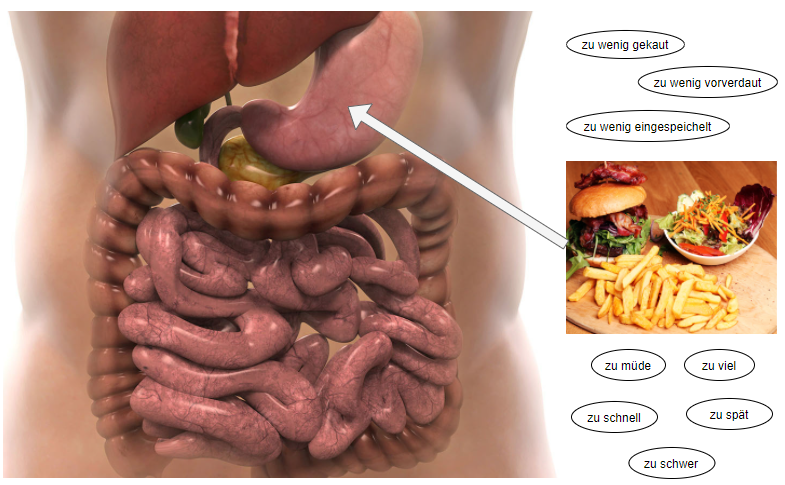
\includegraphics[width=8cm]{../images/vergiftung_1.png}
            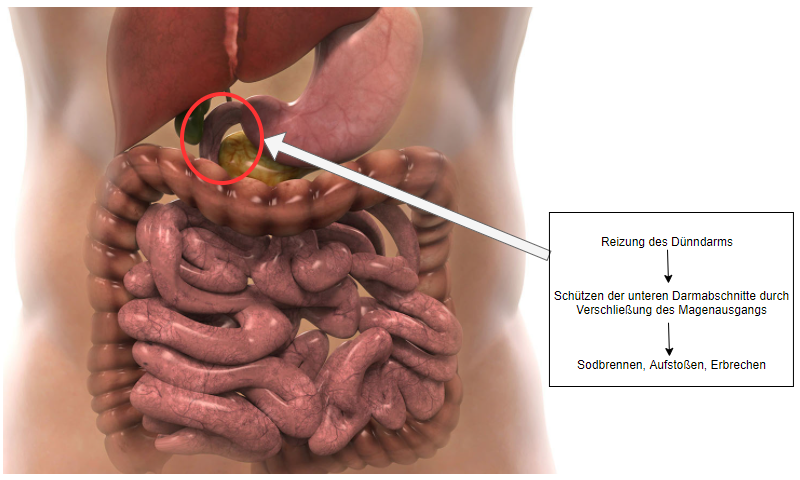
\includegraphics[width=8cm]{../images/vergiftung_2.png}
            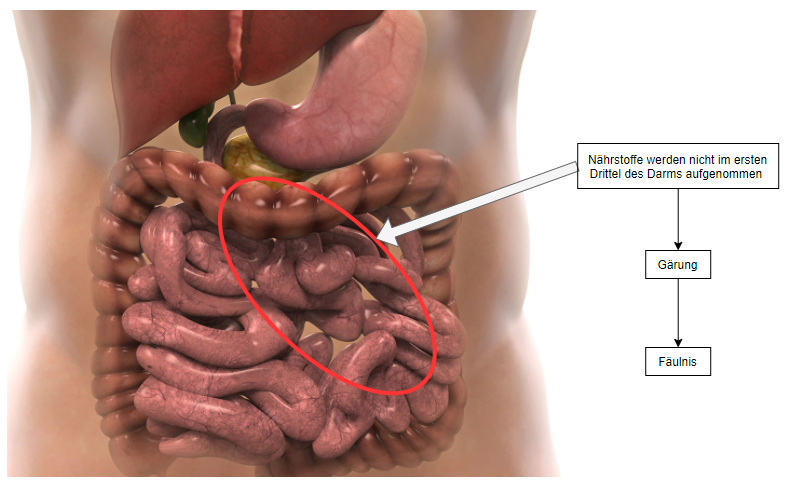
\includegraphics[width=8cm]{../images/vergiftung_3.png}
            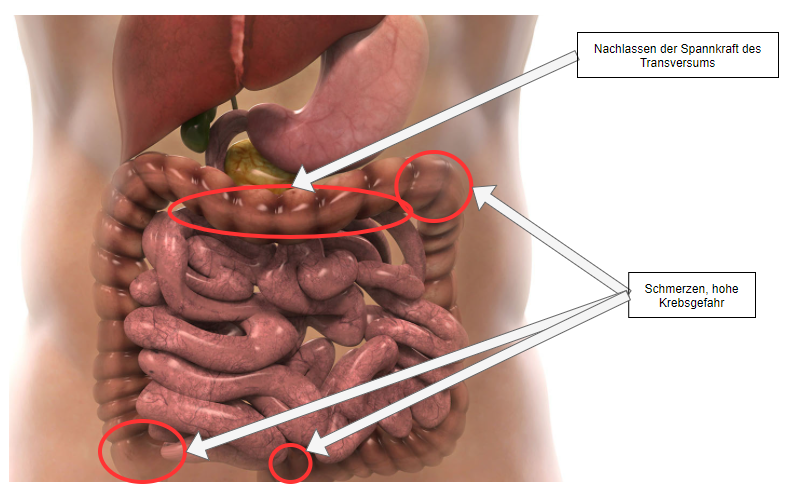
\includegraphics[width=8cm]{../images/vergiftung_4.png}
            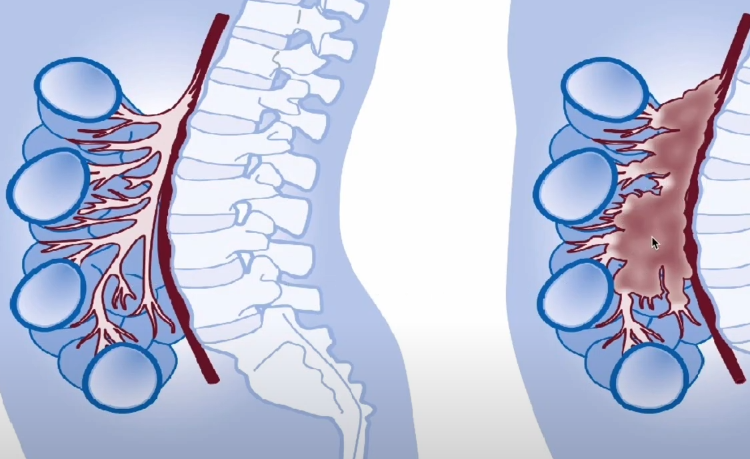
\includegraphics[width=8cm]{../images/lymphe.png}
        \end{figure}
    \end{frame}

    \subsection{Symptome}
    \begin{frame}[allowframebreaks]
        \frametitle{Körperhaltung}

        \begin{figure}
            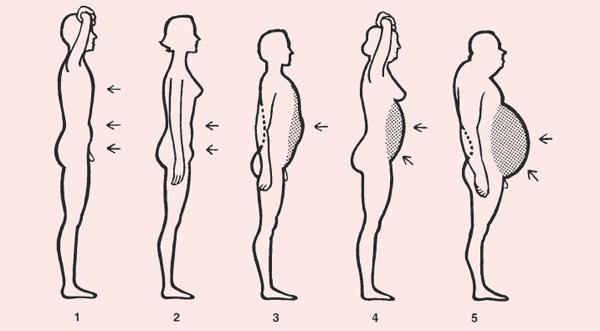
\includegraphics[width=5.4cm]{../images/gasbauch.jpg}\\
            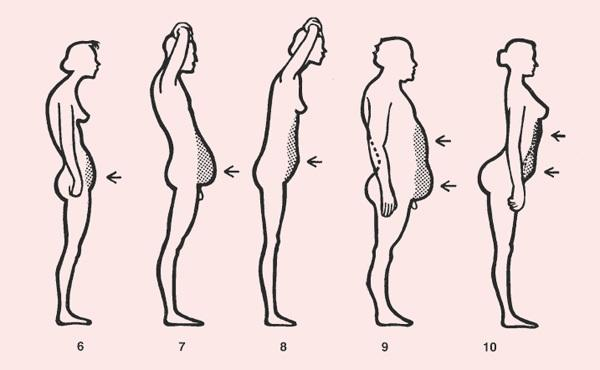
\includegraphics[width=5.4cm]{../images/kotbauch.jpg}
            \caption{Gas- und Kotbäuche}
        \end{figure}

        \begin{itemize}
            \item Normale Lage der Bauchorgane
            \item Normale Größe des Bauchraums
            \item Normale Form der Wirbelsäule
        \end{itemize}

        \begin{figure}
            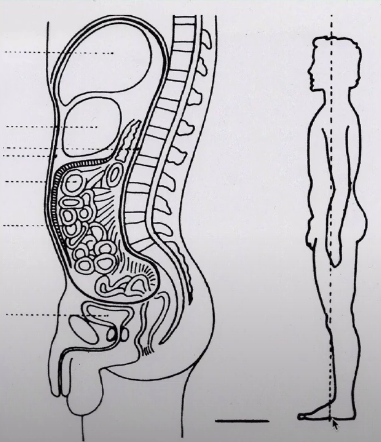
\includegraphics[width=4cm]{../images/normalhaltung.png}
            \caption{Normalhaltung}
        \end{figure}

        \begin{figure}
            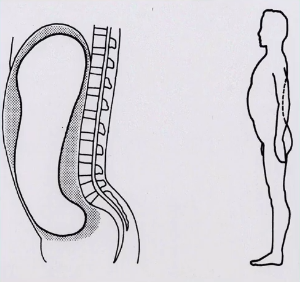
\includegraphics[width=4cm]{../images/habtachthaltung.png}
            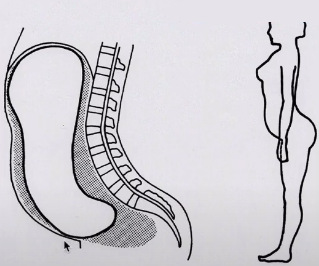
\includegraphics[width=4.5cm]{../images/entenhaltung.png}
            \caption{Aktiver Mann (Habtachthaltung) \& aktive Frau (Entenhaltung)}
        \end{figure}

        \begin{figure}
            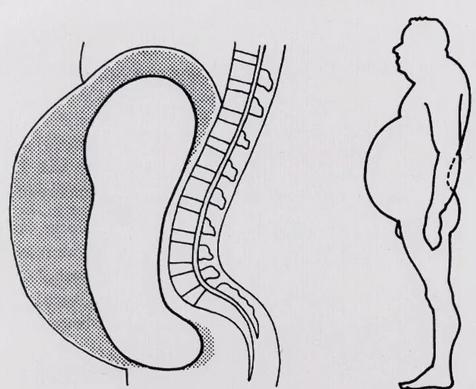
\includegraphics[width=4.7cm]{../images/großtrommelträger.png}
            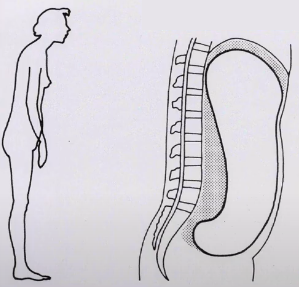
\includegraphics[width=4cm]{../images/anlaufhaltung.png}
            \caption{Großtrommelträger \& Anlaufhaltung (mukelschwächere Menschen)}
        \end{figure}

        \begin{figure}
            \includegraphics[width=3.6cm]{../images/lässige.png}
            \includegraphics[width=4cm]{../images/sämannshaltung.png}
            \caption{Lässige Haltung \& Sämannshaltung}
        \end{figure}
    \end{frame}

    \begin{frame}
        \frametitle{Atmung \& Schulternhöhe}

        \begin{figure}
            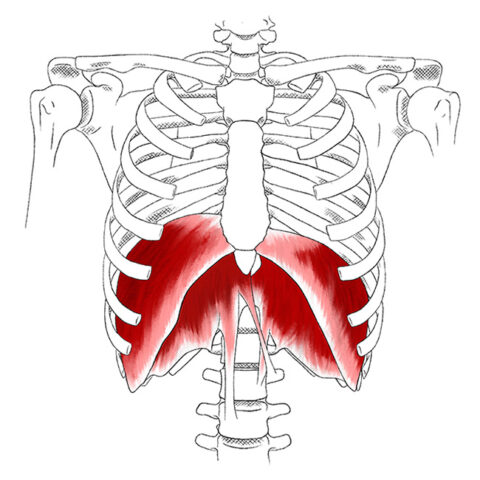
\includegraphics[width=5cm]{../images/therapie_1.jpg}
            \caption{Zwerchfell}
        \end{figure}
    \end{frame}

    \subsection{Kritik}
    \begin{frame}[allowframebreaks]
        \frametitle{Kritik}

        \begin{block}{Säure-Basen-Haushalt}
            \begin{itemize}
                \setlength\itemsep{1em}
                \item $NaCl + CO_{2} + H_{2}O = HCl + NaHCO_3$
                \item Salzsäureproduktion in der Magenwand
                \item Körpereigene Puffersysteme
                \item Kein Einfluss durch säure- oder basenhaltige Nahrungsmittel
            \end{itemize}
        \end{block}

        \begin{block}{Alternativmedizin}
            \begin{itemize}
                \setlength\itemsep{1em}
                \item Orthomolekulare Medizin
                \item hochdosierte Verwendung von Vitaminen, Mineralstoffen, Spurenelementen und Fettsäuren
                \item Kein Nachweis der Wirksamkeit
                \item "`Biochemisches Ungleichgewicht"'
                \item "`Moderne"' Mayr Medizin
            \end{itemize}
        \end{block}
    \end{frame}

    \section{Praxis}
    {
        \setbeamercolor{normal text}{fg=hBlue}\usebeamercolor*{normal text}
        \begin{frame}
            \begin{center}
                \Huge Praxis
            \end{center}
        \end{frame}
    }

    \begin{frame}{Tipps \& Tricks}
        \begin{itemize}
            \setlength\itemsep{1em}
            \item Essensprinzipien einhalten, also nicht
            \begin{itemize}
                \item zu schnell
                \item zu viel
                \item zu oft
                \item zu spät
                \item zu schwer
            \end{itemize}
            \item Bauchmassage: Coecum ascendens, transversum, descendum
            \item Kauen (mal wieder)
        \end{itemize}
    \end{frame}

    \section{Fragerunde}
    {
        \setbeamercolor{normal text}{fg=hBlue}\usebeamercolor*{normal text}
        \begin{frame}
            \begin{center}
                \Huge Fragerunde
            \end{center}
        \end{frame}
    }
\end{document}